\chapter{Metode}

Følgende er fra \cite{Arlow2002}
\section{Unified process}
Unified process (UP) er en softwareudviklingsmetode. 

\subsection{Overordnede principer}

\textbf{Iterativ} metode benyttes ved UP og beskriver en situation hvor projektet brydes ned til mindre subprojekter (iterationer) som gør fremgangsmåden lettere at håndtere og udføre succesfuldt. Hver iteration giver systemet funktionalitet og når iterationen giver en udvidelse af det færdige system betegnes denne inkrementel. På denne måde bygges softwaren trinvist op og som i sidste ende fører til et fuldt funktionelt system. Ved at bryde projektet ned i en serie af iterationer tillader det en fleksibel tilgang til projekt planlægningen sammenlignet med den gamle vandfaldsmodel som er udformet i mere strikse sekvenser.

\textbf{Use case} ligger fundamentet for udviklingen. Formålet med iteration er som regel at udvikle en eller flere use cases.

\textbf{Arkitektur-centreret} beskriver hvordan systemet brydes ned i komponenter, og hvordan disse interagerer og implementeres. 

\textbf{Risiko-drevet} fokuserer på at identificere risici tidligt, hvorved det bliver muligt at identificere hvilke use-cases der vil være optimalt at koncentrere sig om i starten.

\subsection{Iterationer}
Hver iteration indeholder alle elementer i en almindelig software udviklings projekt; planlægning, analyse og design, konstruktion, integration og test, en intern eller ekstern udgivelse. For hver iteration findes der fem kerneelementer:
\begin{itemize}
    \item Krav: Hvad skal systemet kunne?
    \item Analyse: Raffinere og strukturer krav
    \item Design: Realisere krav i et system arkitektur
    \item Implementering: Bygge softwaren
    \item Test: Verificere at implementering virker som ønsket 
\end{itemize}

\subsection{Struktur}
UP er overordnet delt ind i fire faser. Hver fase kan have en eller flere iterationer, og for hver iteration udføres de fem kerneelementer. Mængden af arbejde der lægges i de fem kerneelementer ændres i de forskellige faser i takt med at projektet skrider frem, se figur \ref{fig:UP}.
\begin{itemize}
    \item \textbf{Forberedelse}: De grundlæggende visioner for systemet og et overblik over kravene fastslås. Desuden identificeres risici og formål defineres. 
    \item \textbf{Etablering}: Der fastlægges en grundlæggende arkitektur. Systembeskrivelse og kravspecifikationer defineres. Fokus i etableringsfasen er på krav, analyse og design elementerne. I slutningen af denne fase bliver implementering et vigtigt element, når den grundlæggende arkitektur er produceret.  
    \item \textbf{Konstruktion}: Systemets funktioner udvikles og testes. Målet er at færdiggøre alle krav, analyse og design og udvikle det endelig system. I denne fase vægtes implementeringselementet. 
    \item \textbf{Overdragelse}: Overgangen hvor systemet leveres til slutbrugeren. 
\end{itemize}

\begin{figure}[H]
\centering
  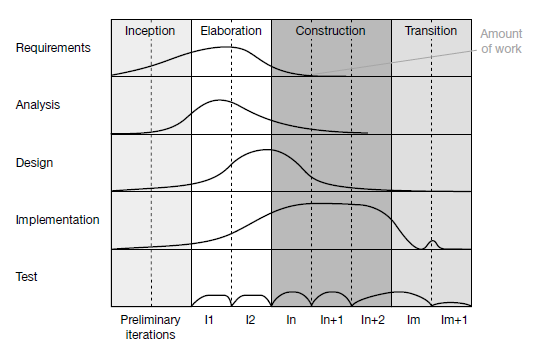
\includegraphics[width=0.8\textwidth]{Billeder/UP.png}
   \caption{Kolonerne i figuren repræsenterer faserne mens rækkerne repræsenterer de fem kerneelementer. Figuren illustrerer hvordan arbejdsfordeling af de fem kerneelementer varierer afhængig af hvilken fase man befinder sig i. \cite{Arlow2002}} 
   \label{fig:UP}
\end{figure}

%Kunne godt tænke mig at komme tænke mig at vide mere om hvad de 5 kerne elementer indebærer 

\section{Objekt orienteret programmering}

%Der findes tre grundprincipper i objektorienteret programmering; indkapsling, nedarving og polymorfi. Et objekt indkapsler nogle data og noget funktionalitet (adfærd). Nedarving. Et objekt kan arve data og funktionalitet fra et andet objekt og udvide med med ekstra data og funktionalitet. Polymorfi. To klasser han kave samme grænseflade defineret via nedarving, men udføre dem forskelligt. Java er et eksempel på et almindeligt objektorienteret sprog og systemet er opbygget af indbyrdes sammemhængende objekter. Der er altid et overordnet objekt som instantierer et andet objekt, dvs. laer sin egen kopi af et andet objekt. 
Objektorienteret programmering er et paradigme indenfor softwareudvikling. Den overordnede filosofi er at definere et softwaresystem bestående af en samling af objekter som interagerer med hinanden.  Programmeringskoden opdeles i klasser, som hver har sit ansvarsområde i programmet. Et objekt er en instans af en klasse og en klasse kan således genbruges adskillige gange til at skabe objekterne. Klassen er en skabelon som definerer objektets adfærd og består overordnet af to delelementer; attributter og metoder. Attributter definerer objektets egenskaber mens metoder definerer de mulige funktioner som objektet kan udføre. \cite{Dathan}  

\section{Unified Modeling Language (UML)}

UML er en standard for diagrammer, som beskriver objektorienteret programmering.

\textbf{Krav} Før analyse og design påbegyndes, er der behov for at kravspecifikationerne defineres. Krav danner basis for systemet og fortæller hvad synes skal kunne gøre. Der findes to typer af krav; de funktionelle kravspecifikationer som udledes ud fa use cases og ikke funktionelle krav som omhandler begrænsinger af systemet. 

\textbf{Use case} Først defineres aktører som direkte interagerer med systemet og findes eksternt for systemet. Derefter opstilles use cases som er noget en aktør ønsker systemet skal kunne gøre. 

\textbf{Analyse} Skabe modeller som fortæller om systemets ønskede adfærd. Producer analyse modeller som fokuserer på hvad systemet skal kunne gøre mens hvordan det skal gøres overlades til design. 

Use case realizations: samarbejdet mellem objekter som viser hvordan integaktion mellem objekter kan realiserer en adfærd udtrykt i use cases. 

Find klasser til objekterne. Klasser består af et sæt af attributer. 

Problem domænet: domæne hvori brugen for et software system opstår. 

\begin{itemize}
    \item Krav: Brugere samt deres behov, hvorudfra der opstilles krav til systemet. Der udarbejdes use cases. Funktionelle og ikke funktionelle krav. 
    \item Analyse: aktivitivitetsdiagrammer for hver use case med forbindelseselementer. Analyseklasse; hvad skal den kunne men ikke hvordan. Analysediagram: hver klasse samt dens egenskab og relation til hinanden. 
    \item Design: Specificer hvordan funktionaliteten kan implementeres. Sekvensdiagrammer; hvordan og hvornår i koden forskellige use cases skal benyttes for at opnå den ønskede funktionalitet. 
    \item Implementering: kodning af de designede modeller. Java. 
    \item Test: test softwarens funktionalitet; white box og black box test. 
\end{itemize}

Brugergrænseflade designprincipper > GUI